\section{Augmented Reality}
In der heutigen Zeit ist fast jedem der Begriff Augmented Reality gel�ufig. Jedoch gibt es im wissenschaftlichen Umfeld keine einheitliche Definition. Georg Klein definiert die \ac{AR} als "`Anreicherung der realen Welt um computergenerierte Zusatzobjekte"'. \cite{KleinG}

Viele Abhandlungen zu diesem Thema beziehen sich auf das "`Reality-Virtuality Continuum"', welches von Milgram, Takemura, Utsumi und Kishino welches in Abbildung \ref{rvc_img} zu sehen ist. Dieses stellt bildlich dar, wie sich eine \ac{AR}-Anwendung einordnen l�sst. Links ist die reale Umgebung (Real Environment) und rechts die Virtuelle Umgebung (Virtual Environment) zu sehen. 

Heutige \ac{VR}-Anwendungen m�ssen also ganz rechts eingeordnet werden. Zwischen der realen und der virtuellen Umgebung gibt es jedoch noch weitere Abstufungen. So gibt es die ?Augmented  Reality?, welche die reale Welt um virtuelle Elemente erg�nzt. Sie bezieht sich eher auch die reale Umgebung, weshalb sie weitere links angeordnet ist. Die ?Augmented Virtuality? ist das genaue Gegenteil der \ac{AR}. Hier wird die virtuelle Welt des Computers um reale Gegenst�nde erg�nzt. 

Im wissenschaftlichen Umfeld wird als Oberbegriff f�r "`Augmented Reality"' und "`Augmented Virtuality"' oft "`Mixed Reality"' oder "`Enhanced Reality"' verwendet. \cite{ARTuP}

\begin{figure}[!ht]
\centering
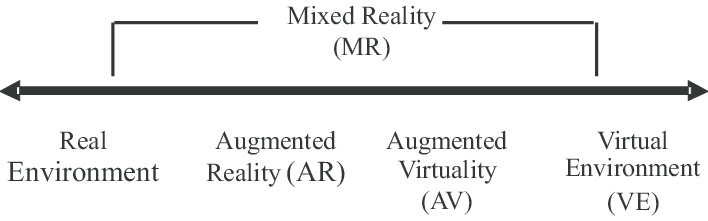
\includegraphics[width=10cm]{Bilder/ar_vr.png}
\caption{Reality-Virtuality Continuum \cite{rvc}}
\label{rvc_img}
\centering
\end{figure}

Der Begriff der \ac{AV} ist heute weniger gebr�uchlich, da es keine wirklichen Anwendungsfelder gibt, in denen eine virtuelle Welt um reale Gegenst�nde erg�nzt werden muss. Im Umkehrschluss wird heute jedoch die \ac{AR} immer bedeutender, da bei fast jeder menschlichen T�tigkeit eine Unterst�tzung durch Computergenerierte Objekte oder Informationen m�glich ist. 

Im medizinischen Umfeld, k�nnen �rzten zum Beispiel Positionen von empfindlichen Gewebe oder zu entfernenden Fremdk�rpern bei einer Operation angezeigt werden. Eine andere Einsatzm�glichkeit w�re das unterst�tzende Anzeigen von Gefahren oder Fluchtwegen f�r Feuerwehrleute, die sich einem stark verrauchten Brandobjekt befinden. Computer k�nnen durch Infrarot und W�rmebild das Sichtverm�gen eines Feuerwehrmannes in einer Gefahrensituation so entscheidend erh�hen um sich selbst und andere zu retten.

\subsection{Typen von visuelle Ausgabeger�te}
Im folgenden Abschnitt werden m�gliche visuelle Ausgabeger�tetypen genauer beschrieben und auf ihre Einsatzm�glichkeiten untersucht. 

\subsubsection{Handheld-Ger�te}

\subsubsection{Video-See-Throuth-Displays}